\documentclass{article}[18pt]
\ProvidesPackage{format}
%Page setup
\usepackage[utf8]{inputenc}
\usepackage[margin=0.7in]{geometry}
\usepackage{parselines} 
\usepackage[english]{babel}
\usepackage{fancyhdr}
\usepackage{titlesec}
\hyphenpenalty=10000

\pagestyle{fancy}
\fancyhf{}
\rhead{Sam Robbins}
\rfoot{Page \thepage}

%Characters
\usepackage{amsmath}
\usepackage{amssymb}
\usepackage{gensymb}
\newcommand{\R}{\mathbb{R}}

%Diagrams
\usepackage{pgfplots}
\usepackage{graphicx}
\usepackage{tabularx}
\usepackage{relsize}
\pgfplotsset{width=10cm,compat=1.9}
\usepackage{float}

%Length Setting
\titlespacing\section{0pt}{14pt plus 4pt minus 2pt}{0pt plus 2pt minus 2pt}
\newlength\tindent
\setlength{\tindent}{\parindent}
\setlength{\parindent}{0pt}
\renewcommand{\indent}{\hspace*{\tindent}}

%Programming Font
\usepackage{courier}
\usepackage{listings}
\usepackage{pxfonts}

%Lists
\usepackage{enumerate}
\usepackage{enumitem}

% Networks Macro
\usepackage{tikz}


% Commands for files converted using pandoc
\providecommand{\tightlist}{%
	\setlength{\itemsep}{0pt}\setlength{\parskip}{0pt}}
\usepackage{hyperref}

% Get nice commands for floor and ceil
\usepackage{mathtools}
\DeclarePairedDelimiter{\ceil}{\lceil}{\rceil}
\DeclarePairedDelimiter{\floor}{\lfloor}{\rfloor}

% Allow itemize to go up to 20 levels deep (just change the number if you need more you madman)
\usepackage{enumitem}
\setlistdepth{20}
\renewlist{itemize}{itemize}{20}

% initially, use dots for all levels
\setlist[itemize]{label=$\cdot$}

% customize the first 3 levels
\setlist[itemize,1]{label=\textbullet}
\setlist[itemize,2]{label=--}
\setlist[itemize,3]{label=*}

% Definition and Important Stuff
% Important stuff
\usepackage[framemethod=TikZ]{mdframed}

\newcounter{theo}[section]\setcounter{theo}{0}
\renewcommand{\thetheo}{\arabic{section}.\arabic{theo}}
\newenvironment{important}[1][]{%
	\refstepcounter{theo}%
	\ifstrempty{#1}%
	{\mdfsetup{%
			frametitle={%
				\tikz[baseline=(current bounding box.east),outer sep=0pt]
				\node[anchor=east,rectangle,fill=red!50]
				{\strut Important};}}
	}%
	{\mdfsetup{%
			frametitle={%
				\tikz[baseline=(current bounding box.east),outer sep=0pt]
				\node[anchor=east,rectangle,fill=red!50]
				{\strut Important:~#1};}}%
	}%
	\mdfsetup{innertopmargin=10pt,linecolor=red!50,%
		linewidth=2pt,topline=true,%
		frametitleaboveskip=\dimexpr-\ht\strutbox\relax
	}
	\begin{mdframed}[]\relax%
		\centering
		}{\end{mdframed}}



\newcounter{lem}[section]\setcounter{lem}{0}
\renewcommand{\thelem}{\arabic{section}.\arabic{lem}}
\newenvironment{defin}[1][]{%
	\refstepcounter{lem}%
	\ifstrempty{#1}%
	{\mdfsetup{%
			frametitle={%
				\tikz[baseline=(current bounding box.east),outer sep=0pt]
				\node[anchor=east,rectangle,fill=blue!20]
				{\strut Definition};}}
	}%
	{\mdfsetup{%
			frametitle={%
				\tikz[baseline=(current bounding box.east),outer sep=0pt]
				\node[anchor=east,rectangle,fill=blue!20]
				{\strut Definition:~#1};}}%
	}%
	\mdfsetup{innertopmargin=10pt,linecolor=blue!20,%
		linewidth=2pt,topline=true,%
		frametitleaboveskip=\dimexpr-\ht\strutbox\relax
	}
	\begin{mdframed}[]\relax%
		\centering
		}{\end{mdframed}}
\lhead{Software Engineering}


\begin{document}
\begin{center}
\underline{\huge Risks}
\end{center}
What is a risk?
\begin{itemize}
	\item Involves choice and uncertainty
	\item Based on incomplete information
\end{itemize}
The "cautious planner" school of risk management:
\begin{itemize}
	\item Identify risks in advance
	\item Assess probability and impact
	\item Prioritise
	\item Risk management plan
\end{itemize}
Types of risk:
\begin{itemize}
	\item Project risks
	\item Technical risks
	\item Business risks
	\item Known risks
	\item Predictable risks
	\item Unknown risks
\end{itemize}


A risk can be measured by its likelihood $\times$ the impact 
\begin{center}
	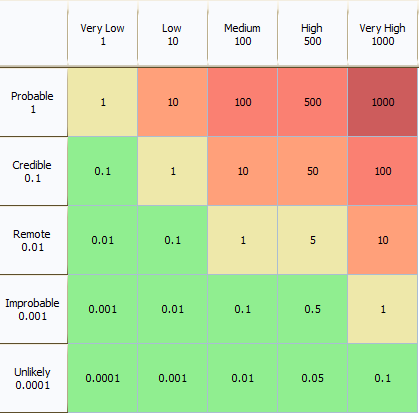
\includegraphics[scale=0.5]{risk}
\end{center}
A risk is an unwanted event that has negative consequences. Project managers must engage in risk management to understand and control the risks on their project\\
\\
Distinguish risks from other project events by looking for:
\begin{enumerate}
	\item Loss associated with the event - risk impact
	\item Likelihood the event will happen - risk probability
	\item Degree to which we can change the outcome - risk control
\end{enumerate}
There are two major sources of risk
\begin{itemize}
	\item Generic risk
	\item Project risk
\end{itemize}
\section{Risk management}
Risk management is concerned with identifying risks and drawing up plans to minimise their effect on a project\\
\\
A risk is a probability that some adverse circumstance will occur, they can be typed:
\begin{itemize}
	\item Project risks affect schedule or resources
	\item Product risks affect the quality or performance of the software being developed
	\item Business risks affect the organisation developing or procuring the software
\end{itemize}
\begin{center}
	\includegraphics[scale=0.5]{"risk management"}
\end{center}
\section{Risk identification}
May be team activities or based on the individual project manager's experience\\
A checklist of common risks may be used to identify risks in a project
\begin{itemize}
	\item Technology risks
	\item People risks
	\item Organisational risks
	\item Tools risk
	\item Requirements risks
	\item Estimation risks
\end{itemize}
\section{Risk analysis}
\begin{itemize}
	\item Asses probability and seriousness of each risk
	\item Probability may be very low, low, moderate, high or very high
	\item Risk consequences might be catastrophic, serious, tolerable or insignificant
\end{itemize}
\section{Risk mitigation}
Consider each risk and develop a strategy to manage that risk:
\begin{itemize}
	\item Avoidance strategies - the probability that the risk will arise is reduced
	\item Minimisation strategies - the impact of the risk on the project or product will be reduced
	\item Contingency plans - if the risk arises, contingency plans are plans to deal with that risk
\end{itemize}
\section{Risk monitoring}
Assess each identified risks regularly to decide whether it is becoming less or more probable\\
\\
Risk monitoring tracks progress
\begin{itemize}
	\item Assess whether a predicted risk occurs
	\item Assess whether the effects of the risk have changed
	\item Ensures that risk aversion steps are defined and properly applied
	\item Collects information that can be used in the future
\end{itemize}
Each key risk should be discussed at management progress meetings\\
When problems occur we need to be able to identify why


\end{document}